\section{Code Changes}
Repository: \url{https://csgitlab.reading.ac.uk/di918039/cs1pr-portfolio}.

Reference the URL of your code repository (that you made accessible to us).
Include a {\texttt diff} of your code repository on CSGitlab from the provided skeleton code; the intital {\texttt commit} (which is the code for Week 1 tutorial) and your final working version.

This can be achieved as follows:
In CSGitlab, go to your repository, select Repository, then Compare.
Now enter as Source "master" and as "target" the Git revision of the initial code and press "Compare".
You will see the history of commits and the detailed changes (deltas) to the original code.
Print this as PDF and include it here.

\textbf{To make this work: after you received the project code, commit the initial code without any changes.}

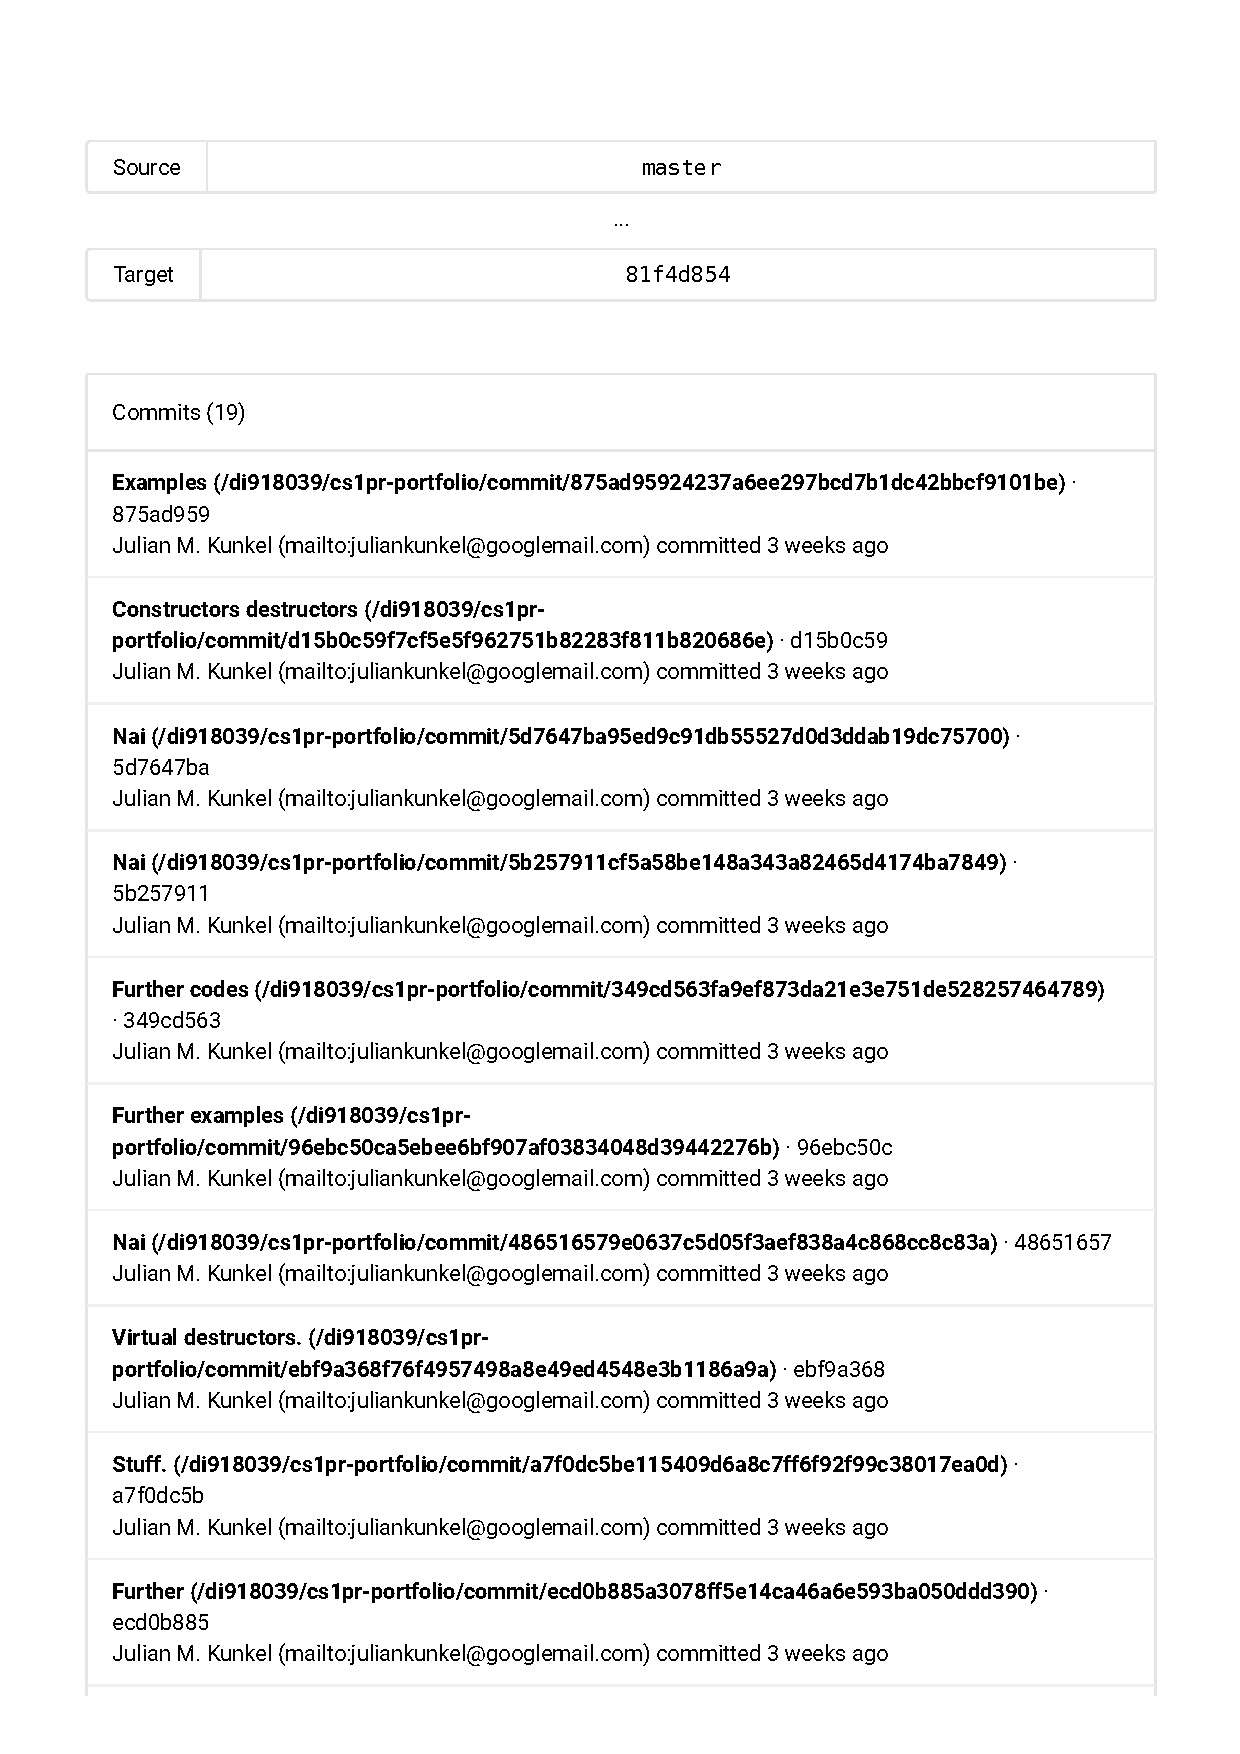
\includepdf[pages=-]{code-delta.pdf}
